\scanpage{71}
\mspage{3}
subgroupoid induced on a \uline{finite} subset \deleted{\illegible{1}} $I$ of $X_K$, one will be able to find a finite number of such generators --- it suffices for example to choose an \deleted{\unsure{$x$}} $x_0\in I$, and choose for every $x\in I\setminus x_0$ a path $l_x$ from $x_0$ to $x$, and in addition a \inserted{finite} system of generators $l_i$ of $\Pi_1(X,x_0)$.

\unsure{It|I} appears that under fairly general conditions (for example if $X$ is an anabelian algebraic curve) knowledge of the action $u$ on $\widehat{\Pi}_1(X_K,I)$ (\inserted{for a} $u\in\Gamma$) \uline{suffices to} determine $u$ --- and the question then arises of seeing how knowledge of the invariants \inserted{say} $g_{l_\alpha}(u)$ (for a generating system of arrows $l_\alpha$ of $\Pi_1(X,I)$) makes it possible to recover the invariants $g_l(u)$ for other \inserted{$K$-}schemes $Y\ldots$.
\margin{\figure{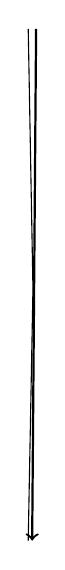
\begin{tikzpicture}[x=1mm,y=1mm]\draw (0,0)--(.6,32)--(0,65);\draw[->,line width=.8pt] (1,65)--(.5,0);\end{tikzpicture}}}

When it is a question of the same scheme $X$, and one is interested in paths $l:x\longrightarrow y$ $(x,y\in I)$ other than the chosen generators $l_\alpha$, the formula gives in principle a means of reconstructing the $g_l(u)$ for every $l$, since it makes it possible to recover the ${}^u l$, and ${}^u l$ is multiplicative in $l$. In terms of the $g_l(u)$, \deleted{$=f_l(u)$}, the multiplicativity formula (6) is written, for a situation
\margin{\uline{NB} for the moment, one only looks at the $x\in X_K$ which are in $I$, the finite system of vertices chosen.}
\diagram{\begin{tikzcd}[ampersand replacement=\&,column sep=large]
x\arrow[r,"l'"] \& y\arrow[r,"{l\deleted{\unsure{''|'}}}"] \& z
\end{tikzcd}}
\[
(10)\qquad \unsure{g_{ll'}(ll'\deleted{u})|g_{ll'}(\deleted{ll'}u)}=g_l(u)\cdot l\bigl(g_{l'}(u)\bigr)
\qquad\text{or }g_u(ll')=g_u(l)\cdot l\bigl(g_u(l')\bigr)
\]
\margin{70}
